\documentclass[tikz,border=4pt]{standalone}
\usepackage[T1]{fontenc}
\usepackage{newtxtext}
\usetikzlibrary{arrows.meta,positioning,fit,backgrounds,calc}

\definecolor{fieldblue}{HTML}{DCEAF7}
\definecolor{densitygreen}{HTML}{E3F0E5}
\definecolor{pipelineorange}{HTML}{F8E6D2}
\definecolor{decisiongold}{HTML}{F5EDC8}
\definecolor{checkgrey}{HTML}{E9ECEF}
\definecolor{ink}{HTML}{263746}

\begin{document}
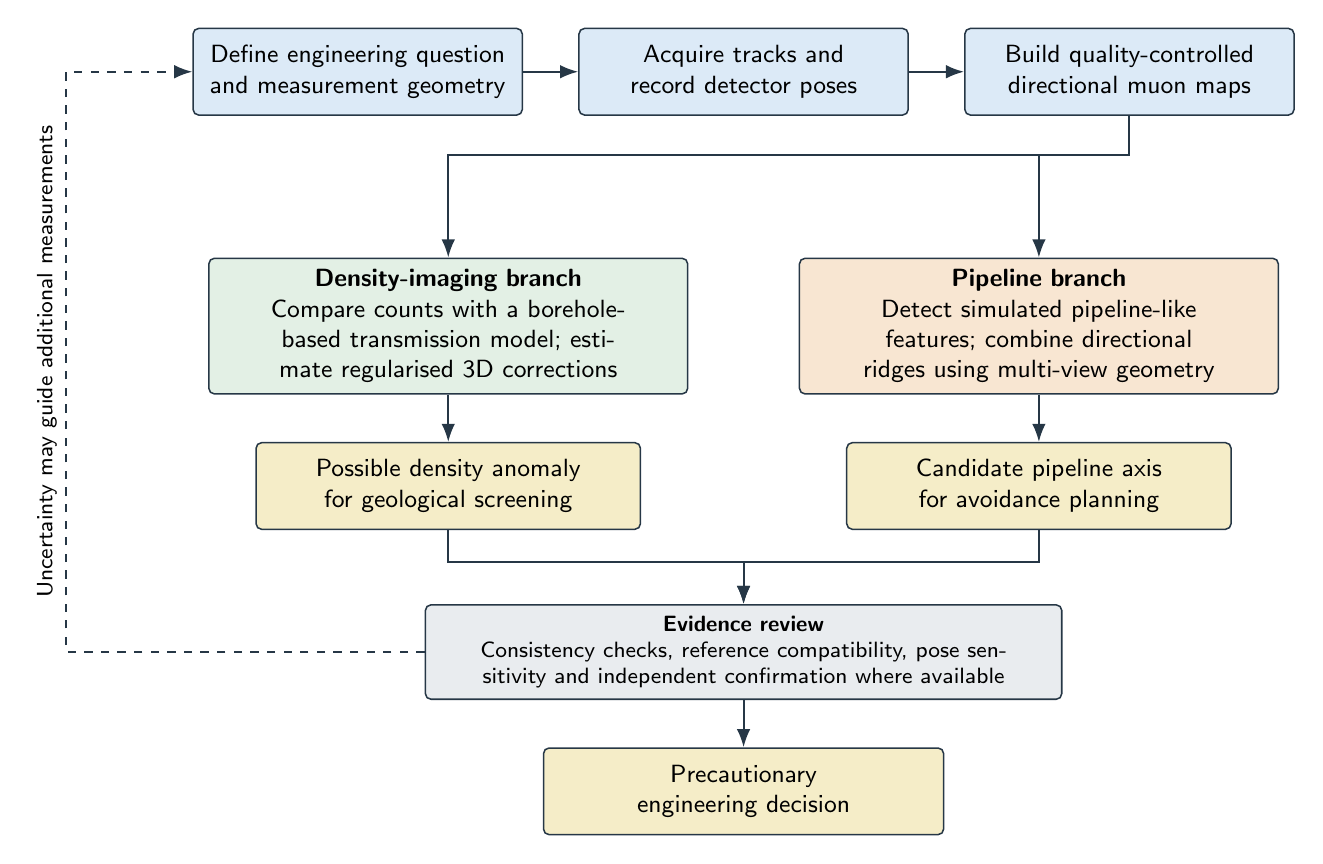
\begin{tikzpicture}[
  font=\sffamily\small,
  >=Latex,
  box/.style={draw=ink, rounded corners=2pt, line width=0.55pt,
    align=center, minimum height=11mm, inner sep=4pt},
  field/.style={box, fill=fieldblue, text width=39mm},
  density/.style={box, fill=densitygreen, text width=58mm},
  pipeline/.style={box, fill=pipelineorange, text width=58mm},
  decision/.style={box, fill=decisiongold, text width=46mm},
  check/.style={box, fill=checkgrey, text width=78mm, font=\sffamily\footnotesize},
  arrow/.style={-{Latex[length=2.3mm]}, line width=0.75pt, draw=ink},
  feedback/.style={-{Latex[length=2.3mm]}, dashed, line width=0.7pt, draw=ink}
]

\node[field] (plan) {Define engineering question\\and measurement geometry};
\node[field, right=7mm of plan] (measure) {Acquire tracks and\\record detector poses};
\node[field, right=7mm of measure] (map) {Build quality-controlled\\directional muon maps};
\draw[arrow] (plan) -- (measure);
\draw[arrow] (measure) -- (map);

\node[density, below left=18mm and -14mm of measure] (density)
  {\textbf{Density-imaging branch}\\Compare counts with a borehole-based transmission model; estimate regularised 3D corrections};
\node[pipeline, below right=18mm and -14mm of measure] (pipeline)
  {\textbf{Pipeline branch}\\Detect simulated pipeline-like features; combine directional ridges using multi-view geometry};

\node[decision, below=6mm of density] (screen) {Possible density anomaly\\for geological screening};
\node[decision, below=6mm of pipeline] (axis) {Candidate pipeline axis\\for avoidance planning};

\node[check, below=15mm of $(screen)!0.5!(axis)$] (review)
  {\textbf{Evidence review}\\Consistency checks, reference compatibility, pose sensitivity and independent confirmation where available};
\node[decision, below=6mm of review, text width=48mm] (action)
  {Precautionary\\engineering decision};

\draw[arrow] (map.south) -- ++(0,-5mm) -| (density.north);
\draw[arrow] (map.south) -- ++(0,-5mm) -| (pipeline.north);
\draw[arrow] (density) -- (screen);
\draw[arrow] (pipeline) -- (axis);
\draw[arrow] (screen.south) -- ++(0,-4mm) -| (review.north);
\draw[arrow] (axis.south) -- ++(0,-4mm) -| (review.north);
\draw[arrow] (review) -- (action);

\coordinate (fb1) at ([xshift=-18mm]density.west |- review.west);
\coordinate (fb2) at (fb1 |- plan.west);
\draw[feedback] (review.west) -- (fb1) -- (fb2) -- (plan.west);
\node[font=\sffamily\footnotesize, rotate=90, anchor=south]
  at ($(fb1)!0.5!(fb2)$) {Uncertainty may guide additional measurements};

\end{tikzpicture}
\end{document}
